%\documentclass{article}
%\usepackage{graphicx,subfigure}
%\begin{document}

\begin{figure}[!h]
  \centering
  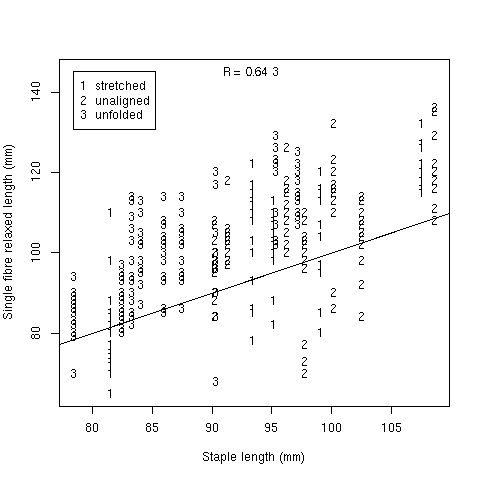
\includegraphics[width=1.0\textwidth]{figLrLs.png}
%   15fibreLsLr.png is original 
  \caption{Plot of staple length against relaxed fibre length for fibres removed from staples for the SF technique. There are 15 fibres per sheep, one staple per sheep, and 21 sheep}
\label{fig:LrLs}
\end{figure}

%\end{document}

